\documentclass[DIV=14,titlepage=false]{scrreprt}
\usepackage{parskip}
%%%%%%%%%%%%%%%%%%%%%%%%%%%%%%%%%%%%%%%%%%%%%%%%%%%%%%%%%%%%%%%%%%%%%%%%%%%%%%%
%                                Basic Packages                               %
%%%%%%%%%%%%%%%%%%%%%%%%%%%%%%%%%%%%%%%%%%%%%%%%%%%%%%%%%%%%%%%%%%%%%%%%%%%%%%%
% Gives us multiple colors.
\usepackage[usenames,dvipsnames,pdftex]{xcolor}
% Lets us style link colors.
\usepackage{hyperref}
% Lets us import images and graphics.
\usepackage{graphicx}
% Lets us use figures in floating environments.
\usepackage{float}
% Lets us create multiple columns.
\usepackage{multicol}
% Gives us better math syntax.
\usepackage{amsmath,amsfonts,mathtools,amsthm,amssymb}
% Lets us strikethrough text.
\usepackage{cancel}
% Lets us edit the caption of a figure.
\usepackage{caption}
% Lets us import pdf directly in our tex code.
\usepackage{pdfpages}
% Lets us do algorithm stuff.
\usepackage[ruled,vlined,linesnumbered]{algorithm2e}
% Gets rid of some errors.
\usepackage{scrhack}
\def\class{article}
\usepackage{geometry}
\geometry{margin=0.9in}
%%%%%%%%%%%%%%%%%%%%%%%%%%%%%%%%%%%%%%%%%%%%%%%%%%%%%%%%%%%%%%%%%%%%%%%%%%%%%%%
%                                Basic Settings                               %
%%%%%%%%%%%%%%%%%%%%%%%%%%%%%%%%%%%%%%%%%%%%%%%%%%%%%%%%%%%%%%%%%%%%%%%%%%%%%%%

%%%%%%%%%%%%%
%  Symbols  %
%%%%%%%%%%%%%

\let\implies\Rightarrow
\let\impliedby\Leftarrow
\let\iff\Leftrightarrow
\let\epsilon\varepsilon

%%%%%%%%%%%%
%  Tables  %
%%%%%%%%%%%%

\setlength{\tabcolsep}{5pt}
\renewcommand\arraystretch{1.5}

%%%%%%%%%%%%%%%%%%%%%%%
%  Center Title Page  %
%%%%%%%%%%%%%%%%%%%%%%%

\usepackage{titling}
\renewcommand\maketitlehooka{\null\mbox{}\vfill}
\renewcommand\maketitlehookd{\vfill\null}

%%%%%%%%%%%%%%%%%%%%%%%%%%%%%%%%%%%%%%%%%%%%%%%%%%%%%%%
%  Create a grey background in the middle of the PDF  %
%%%%%%%%%%%%%%%%%%%%%%%%%%%%%%%%%%%%%%%%%%%%%%%%%%%%%%%

\usepackage{eso-pic}
\newcommand\definegraybackground{
  \definecolor{reallylightgray}{HTML}{FAFAFA}
  \AddToShipoutPicture{
    \ifthenelse{\isodd{\thepage}}{
      \AtPageLowerLeft{
        \put(\LenToUnit{\dimexpr\paperwidth-222pt},0){
          \color{reallylightgray}\rule{222pt}{297mm}
        }
      }
    }
    {
      \AtPageLowerLeft{
        \color{reallylightgray}\rule{222pt}{297mm}
      }
    }
  }
}

%%%%%%%%%%%%%%%%%%%%%%%%
%  Modify Links Color  %
%%%%%%%%%%%%%%%%%%%%%%%%

\hypersetup{
  % Enable highlighting links.
  colorlinks,
  % Change the color of links to blue.
  linkcolor={black},
  % Change the color of citations to black.
  citecolor={black},
  % Change the color of url's to blue with some black.
  urlcolor=blue
}

%%%%%%%%%%%%%%%%%%
% Fix WrapFigure %
%%%%%%%%%%%%%%%%%%

\newcommand{\wrapfill}{\par\ifnum\value{WF@wrappedlines}>0
    \parskip=0pt
    \addtocounter{WF@wrappedlines}{-1}%
    \null\vspace{\arabic{WF@wrappedlines}\baselineskip}%
    \WFclear
\fi}

%%%%%%%%%%%%%%%%%
% Multi Columns %
%%%%%%%%%%%%%%%%%

\let\multicolmulticols\multicols
\let\endmulticolmulticols\endmulticols

\RenewDocumentEnvironment{multicols}{mO{}}
{%
  \ifnum#1=1
    #2%
  \else % More than 1 column
    \multicolmulticols{#1}[#2]
  \fi
}
{%
  \ifnum#1=1
\else % More than 1 column
  \endmulticolmulticols
\fi
}

\newlength{\thickarrayrulewidth}
\setlength{\thickarrayrulewidth}{5\arrayrulewidth}

%%%%%%%%%%%%%%%%%%%%
%  Import Figures  %
%%%%%%%%%%%%%%%%%%%%

\usepackage{import}
\pdfminorversion=7

% EXAMPLE:
% 1. \incfig{limit-graph}
% 2. \incfig[0.4]{limit-graph}
% Parameters:
% 1. The figure name. It should be located in figures/NAME.tex_pdf.
% 2. (Optional) The width of the figure. Example: 0.5, 0.35.
\newcommand\incfig[2][1]{%
  \def\svgwidth{#1\columnwidth}
  \import{./figures/}{#2.pdf_tex}
}

\begingroup\expandafter\expandafter\expandafter\endgroup
\expandafter\ifx\csname pdfsuppresswarningpagegroup\endcsname\relax
\else
  \pdfsuppresswarningpagegroup=1\relax
\fi

%%%%%%%%%%%%%
%  Correct  %
%%%%%%%%%%%%%

% EXAMPLE:
% 1. \correct{INCORRECT}{CORRECT}
% Parameters:
% 1. The incorrect statement.
% 2. The correct statement.
\definecolor{correct}{HTML}{009900}
\newcommand\correct[2]{{\color{red}{#1 }}\ensuremath{\to}{\color{correct}{ #2}}}



\newcommand{\R}{\mathbb{R}}
\newcommand{\Z}{\mathbb{Z}}
\newcommand{\E}{\mathbb{E}}
\newcommand{\B}{\ensuremath{\mathcal{B}}}
\newcommand{\X}{\ensuremath{\mathcal{X}}}
\newcommand{\Y}{\ensuremath{\mathcal{Y}}}
\newcommand{\mA}{\ensuremath{\mathbf{A}}}
\newcommand{\mB}{\ensuremath{\mathbf{B}}}
\newcommand{\mC}{\ensuremath{\mathbf{C}}}
\newcommand{\mD}{\ensuremath{\mathbf{D}}}
\newcommand{\mX}{\ensuremath{\mathbf{X}}}
\newcommand{\mY}{\ensuremath{\mathbf{Y}}}
\newcommand{\mx}{\ensuremath{\mathbf{x}}}
\newcommand{\my}{\ensuremath{\mathbf{y}}}
\newcommand{\mI}{\ensuremath{\mathbf{I}}}
\newcommand{\mi}{\ensuremath{\mathbf{\iota}}}
\newcommand{\mmu}{\ensuremath{\mathbf{\mu}}}
\newcommand{\mc}{\ensuremath{\mathbf{c}}}
\newcommand{\mSigma}{\ensuremath{\mathbf{\Sigma}}}
\newcommand{\mzero}{\ensuremath{\mathbf{0}}}
\newcommand{\independent}{\perp\!\!\!\!\perp} 
\setlength{\parindent}{0pt}
%%%%%%%%%%%%%%%%%%%%%%%%%%%%%%%%%%%%%%%%%%%%%%%%%%%%%%%%%%%%%%%%%%%%%%%%%%%%%%%
%                                 Environments                                %
%%%%%%%%%%%%%%%%%%%%%%%%%%%%%%%%%%%%%%%%%%%%%%%%%%%%%%%%%%%%%%%%%%%%%%%%%%%%%%%

\usepackage{varwidth}
\usepackage{thmtools}
\usepackage[most,many,breakable]{tcolorbox}

\tcbuselibrary{theorems,skins,hooks}
\usetikzlibrary{arrows,calc,shadows.blur}

%%%%%%%%%%%%%%%%%%%
%  Define Colors  %
%%%%%%%%%%%%%%%%%%%

\definecolor{myblue}{RGB}{45, 111, 177}
\definecolor{mygreen}{RGB}{56, 140, 70}
\definecolor{myred}{RGB}{199, 68, 64}
\definecolor{mypurple}{RGB}{197, 92, 212}

\definecolor{definition}{HTML}{228b22}
\definecolor{theorem}{HTML}{00007B}
\definecolor{example}{HTML}{2A7F7F}
\definecolor{definition}{HTML}{228b22}
\definecolor{prop}{HTML}{191971}
\definecolor{lemma}{HTML}{983b0f}
\definecolor{exercise}{HTML}{88D6D1}

\colorlet{definition}{mygreen!85!black}
\colorlet{claim}{mygreen!85!black}
\colorlet{corollary}{mypurple!85!black}
\colorlet{proof}{theorem}

%%%%%%%%%%%%%%%%%%%%%%
%  Helpful Commands  %
%%%%%%%%%%%%%%%%%%%%%%

% EXAMPLE:
% 1. \createnewtheoremstyle{thmdefinitionbox}{}{}
% 2. \createnewtheoremstyle{thmtheorembox}{}{}
% 3. \createnewtheoremstyle{thmproofbox}{qed=\qedsymbol}{
%       rightline=false, topline=false, bottomline=false
%    }
% Parameters:
% 1. Theorem name.
% 2. Any extra parameters to pass directly to declaretheoremstyle.
% 3. Any extra parameters to pass directly to mdframed.
\newcommand\createnewtheoremstyle[3]{
  \declaretheoremstyle[
  headfont=\bfseries\sffamily, bodyfont=\normalfont, #2,
  mdframed={
    #3,
  },
  ]{#1}
}

% EXAMPLE:
% 1. \createnewcoloredtheoremstyle{thmdefinitionbox}{definition}{}{}
% 2. \createnewcoloredtheoremstyle{thmexamplebox}{example}{}{
%       rightline=true, leftline=true, topline=true, bottomline=true
%     }
% 3. \createnewcoloredtheoremstyle{thmproofbox}{proof}{qed=\qedsymbol}{backgroundcolor=white}
% Parameters:
% 1. Theorem name.
% 2. Color of theorem.
% 3. Any extra parameters to pass directly to declaretheoremstyle.
% 4. Any extra parameters to pass directly to mdframed.
\newcommand\createnewcoloredtheoremstyle[4]{
  \declaretheoremstyle[
  headfont=\bfseries\sffamily\color{#2}, bodyfont=\normalfont, #3,
  mdframed={
    linewidth=2pt,
    rightline=false, leftline=true, topline=false, bottomline=false,
    linecolor=#2, backgroundcolor=#2!5, #4,
  },
  ]{#1}
}

%%%%%%%%%%%%%%%%%%%%%%%%%%%%%%%%%%%
%  Create the Environment Styles  %
%%%%%%%%%%%%%%%%%%%%%%%%%%%%%%%%%%%

\makeatletter
\@ifclasswith\class{nocolor}{
  % Environments without color.

  \createnewtheoremstyle{thmdefinitionbox}{}{}
  \createnewtheoremstyle{thmtheorembox}{}{}
  \createnewtheoremstyle{thmexamplebox}{}{}
  \createnewtheoremstyle{thmclaimbox}{}{}
  \createnewtheoremstyle{thmcorollarybox}{}{}
  \createnewtheoremstyle{thmpropbox}{}{}
  \createnewtheoremstyle{thmlemmabox}{}{}
  \createnewtheoremstyle{thmexercisebox}{}{}
  \createnewtheoremstyle{thmdefinitionbox}{}{}
  \createnewtheoremstyle{thmquestionbox}{}{}
  \createnewtheoremstyle{thmsolutionbox}{}{}

  \createnewtheoremstyle{thmproofbox}{qed=\qedsymbol}{}
  \createnewtheoremstyle{thmexplanationbox}{}{}
}{
  % Environments with color.

  \createnewcoloredtheoremstyle{thmdefinitionbox}{definition}{}{}
  \createnewcoloredtheoremstyle{thmtheorembox}{theorem}{}{}
  \createnewcoloredtheoremstyle{thmexamplebox}{example}{}{
    rightline=true, leftline=true, topline=true, bottomline=true
  }
  \createnewcoloredtheoremstyle{thmclaimbox}{claim}{}{}
  \createnewcoloredtheoremstyle{thmcorollarybox}{corollary}{}{}
  \createnewcoloredtheoremstyle{thmpropbox}{prop}{}{}
  \createnewcoloredtheoremstyle{thmlemmabox}{lemma}{}{}
  \createnewcoloredtheoremstyle{thmexercisebox}{exercise}{}{}

  \createnewcoloredtheoremstyle{thmproofbox}{proof}{qed=\qedsymbol}{backgroundcolor=white}
  \createnewcoloredtheoremstyle{thmexplanationbox}{example}{qed=\qedsymbol}{backgroundcolor=white}
}
\makeatother

%%%%%%%%%%%%%%%%%%%%%%%%%%%%%
%  Create the Environments  %
%%%%%%%%%%%%%%%%%%%%%%%%%%%%%

\declaretheorem[numberwithin=section, style=thmtheorembox,     name=Theorem]{theorem}
\declaretheorem[numbered=no,          style=thmexamplebox,     name=Example]{example}
\declaretheorem[numberwithin=section, style=thmclaimbox,       name=Claim]{claim}
\declaretheorem[numberwithin=section, style=thmcorollarybox,   name=Corollary]{corollary}
\declaretheorem[numberwithin=section, style=thmpropbox,        name=Proposition]{prop}
\declaretheorem[numberwithin=section, style=thmlemmabox,       name=Lemma]{lemma}
\declaretheorem[numberwithin=section, style=thmexercisebox,    name=Exercise]{exercise}
\declaretheorem[numbered=no,          style=thmproofbox,       name=Proof]{replacementproof}
\declaretheorem[numbered=no,          style=thmexplanationbox, name=Proof]{expl}

\makeatletter
\@ifclasswith\class{nocolor}{
  % Environments without color.

  \newtheorem*{note}{Note}

  \declaretheorem[numberwithin=section, style=thmdefinitionbox, name=Definition]{definition}
  \declaretheorem[numberwithin=section, style=thmquestionbox,   name=Question]{question}
  \declaretheorem[numberwithin=section, style=thmsolutionbox,   name=Solution]{solution}
}{
  % Environments with color.

  \newtcbtheorem[number within=section]{Definition}{Definition}{
    enhanced,
    before skip=2mm,
    after skip=2mm,
    colback=red!5,
    colframe=red!80!black,
    colbacktitle=red!75!black,
    boxrule=0.5mm,
    attach boxed title to top left={
      xshift=1cm,
      yshift*=1mm-\tcboxedtitleheight
    },
    varwidth boxed title*=-3cm,
    boxed title style={
      interior engine=empty,
      frame code={
        \path[fill=tcbcolback]
        ([yshift=-1mm,xshift=-1mm]frame.north west)
        arc[start angle=0,end angle=180,radius=1mm]
        ([yshift=-1mm,xshift=1mm]frame.north east)
        arc[start angle=180,end angle=0,radius=1mm];
        \path[left color=tcbcolback!60!black,right color=tcbcolback!60!black,
        middle color=tcbcolback!80!black]
        ([xshift=-2mm]frame.north west) -- ([xshift=2mm]frame.north east)
        [rounded corners=1mm]-- ([xshift=1mm,yshift=-1mm]frame.north east)
        -- (frame.south east) -- (frame.south west)
        -- ([xshift=-1mm,yshift=-1mm]frame.north west)
        [sharp corners]-- cycle;
      },
    },
    fonttitle=\bfseries,
    title={#2},
    #1
  }{def}

  \NewDocumentEnvironment{definition}{O{}O{}}
    {\begin{Definition}{#1}{#2}}{\end{Definition}}

  \newtcolorbox{note}[1][]{%
    enhanced jigsaw,
    colback=gray!20!white,%
    colframe=gray!80!black,
    size=small,
    boxrule=1pt,
    title=\textbf{Note:-},
    halign title=flush center,
    coltitle=black,
    breakable,
    drop shadow=black!50!white,
    attach boxed title to top left={xshift=1cm,yshift=-\tcboxedtitleheight/2,yshifttext=-\tcboxedtitleheight/2},
    minipage boxed title=1.5cm,
    boxed title style={%
      colback=white,
      size=fbox,
      boxrule=1pt,
      boxsep=2pt,
      underlay={%
        \coordinate (dotA) at ($(interior.west) + (-0.5pt,0)$);
        \coordinate (dotB) at ($(interior.east) + (0.5pt,0)$);
        \begin{scope}
          \clip (interior.north west) rectangle ([xshift=3ex]interior.east);
          \filldraw [white, blur shadow={shadow opacity=60, shadow yshift=-.75ex}, rounded corners=2pt] (interior.north west) rectangle (interior.south east);
        \end{scope}
        \begin{scope}[gray!80!black]
          \fill (dotA) circle (2pt);
          \fill (dotB) circle (2pt);
        \end{scope}
      },
    },
    #1,
  }

  \newtcbtheorem{Question}{Question}{enhanced,
    breakable,
    colback=white,
    colframe=myblue!80!black,
    attach boxed title to top left={yshift*=-\tcboxedtitleheight},
    fonttitle=\bfseries,
    title=\textbf{Question:-},
    boxed title size=title,
    boxed title style={%
      sharp corners,
      rounded corners=northwest,
      colback=tcbcolframe,
      boxrule=0pt,
    },
    underlay boxed title={%
      \path[fill=tcbcolframe] (title.south west)--(title.south east)
      to[out=0, in=180] ([xshift=5mm]title.east)--
      (title.center-|frame.east)
      [rounded corners=\kvtcb@arc] |-
      (frame.north) -| cycle;
    },
    #1
  }{def}

  \NewDocumentEnvironment{question}{O{}O{}}
  {\begin{Question}{#1}{#2}}{\end{Question}}

  \newtcolorbox{Solution}{enhanced,
    breakable,
    colback=white,
    colframe=mygreen!80!black,
    attach boxed title to top left={yshift*=-\tcboxedtitleheight},
    title=\textbf{Solution:-},
    boxed title size=title,
    boxed title style={%
      sharp corners,
      rounded corners=northwest,
      colback=tcbcolframe,
      boxrule=0pt,
    },
    underlay boxed title={%
      \path[fill=tcbcolframe] (title.south west)--(title.south east)
      to[out=0, in=180] ([xshift=5mm]title.east)--
      (title.center-|frame.east)
      [rounded corners=\kvtcb@arc] |-
      (frame.north) -| cycle;
    },
  }

  \NewDocumentEnvironment{solution}{O{}O{}}
  {\vspace{-10pt}\begin{Solution}{#1}{#2}}{\end{Solution}}
}
\makeatother

%%%%%%%%%%%%%%%%%%%%%%%%%%%%
%  Edit Proof Environment  %
%%%%%%%%%%%%%%%%%%%%%%%%%%%%

\renewenvironment{proof}[1][\proofname]{\vspace{-10pt}\begin{replacementproof}}{\end{replacementproof}}
\newenvironment{explanation}[1][\proofname]{\vspace{-10pt}\begin{expl}}{\end{expl}}

\theoremstyle{definition}

\newtheorem*{notation}{Notation}
\newtheorem*{previouslyseen}{As previously seen}
\newtheorem*{problem}{Problem}
\newtheorem*{observe}{Observe}
\newtheorem*{property}{Property}
\newtheorem*{intuition}{Intuition}



\title{%
R300 Econometrics}
\author{Metrics Enjoyers}
\date{Michaelmas Term, 2023-2024}

\setuptoc{toc}{leveldown}
\setcounter{chapter}{10}

\begin{document}
\pagenumbering{gobble}
\chapter{ML Asymptotics. Likelihood Ratio Test.}

More rigour: Amemiya (1985)

\subsection{Consistency of ML}

Let \(z_i\) be iid with density \(f(z;\theta_0)\) for \(i=1,\dots,n\).
\[\hat{\theta}_{ML}=\operatorname*{argmax}_{\theta}\sum_{i=1}^n\log f(z_i;\theta)\]
By Khinchine's LLN for any \(\theta\)
\[\frac{1}{n}\sum_{i=1}^n\log f(z_i;\theta)\xrightarrow{p}\E_{\theta_0}[\log f(z;\theta)]\]
We can invoke KLLN as given \(z_i\) iid \(\implies\) any function of \(z_i\) is also iid. We also need to assume the expectation exists. This is taken over the value of the true parameter, but the conditioned \(\theta\) runs across the real line.
\vspace{5mm}
\begin{prop}
\[\hat{\theta}_{ML}\xrightarrow{p}\operatorname*{argmax}_{\theta}\E_{\theta_0}[\log f(z;\theta)]\]
\end{prop}
\vspace{5mm}
\begin{proof}
\[\hat{\theta}_{ML}=\operatorname*{argmax}_{\theta}\sum_{i=1}^n\log f(z_i;\theta)=\operatorname*{argmax}_{\theta}\frac{1}{n}\sum_{i=1}^n\log f(z_i;\theta)\]
But:
\[\frac{1}{n}\sum_{i=1}^n\log f(z_i;\theta)\xrightarrow{p}\E_{\theta_0}[\log f(z;\theta)] \,\text{\underline{uniformly}} \implies \operatorname*{argmax}_{\theta}\frac{1}{n}\sum_{i=1}^n\log f(z_i;\theta)\xrightarrow{p}\operatorname*{argmax}_{\theta}\E_{\theta_0}[\log f(z;\theta)] \]
\end{proof}
\begin{center}
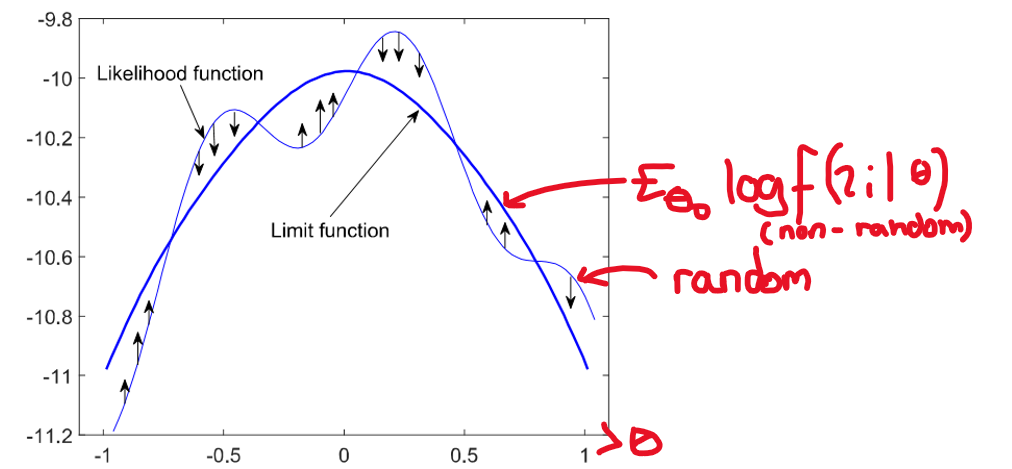
\includegraphics[width=\textwidth]{./Images/ML Asymptotics.png}
\end{center}
\vspace{5mm}
\begin{prop}
    \(E_{\theta_0}\log f(z_i;\theta) \, \text{is maximised at the true value of parameter}\, \theta_0\)
\end{prop}
\vspace{5mm}
\begin{proof}
    Consider the KL divergence between \(f(z;\theta)\) and \(f(z;\theta_0)\):
    \[E_{\theta_0}\log \frac{f(z;\theta_0)}{f(z;\theta)}\]
    By construction the minimiser of the KL divergence must be the maximiser of \(E_{\theta_0}\log f(z;\theta)\).
    By Jensen's inequality:
    \[=-E_{\theta_0}\frac{\log f(z;\theta)}{\log f(z;\theta_0)}\geq-\log E_{\theta_0}\frac{ f(z;\theta)}{f(z;\theta_0)}=-\log\int\frac{f(z;\theta)}{f(z;\theta_0)}f(z;\theta_0)dz=-\log 1 = 0\]
    But we can achieve this bound by setting \(\theta=\theta_0\) is \underline{a} maximiser of \(E_{\theta_0}\log f(z;\theta)\). 
\end{proof}

\begin{note}
If there exists another maximiser \(\theta_1\), we must have \(f(z;\theta_0)=f(z;\theta_1)\) for all \(z\).
In such a case, we say that a case, we say that the parameter is \underline{non-identified}.
\\
In the linear regression example , \(\theta=(\beta',\sigma^2)\), would not be identified if \(X'X\) has rank lower than \(k\) (perfect multicollinearity).

Pointwise convergence is not enough for consistency of the \(\theta_{ML}\) estimator. Sufficient conditions are given by uniform convergence and "enough" curvature of \(E_{\theta_0}\log f(z;\theta)\) around \(\theta_0\).
\end{note}

\subsection{Asymptotic Normality of ML}

\begin{prop}
\[\sqrt{n}(\hat{\theta}_{ML}-\theta_0)\xrightarrow{d}N(0,I^{-1}(\theta_0))\]
where \(I(\theta_0)\) is the Fisher information matrix:
\[I_1(\theta_0)=Var\left[\frac{\partial}{\partial\theta}\log f(z;\theta_0)\right]=-\E\left[\frac{\partial^2}{\partial\theta^2}\log f(z;\theta_0)\right]=E_{\theta_0}(H_1)=\E_{\theta_0}(\frac{H}{n})\]
Note \(I_1(\theta_0)\) is the Fisher information for a single observation.
\\ Define \(I(\theta_0)\) as the Fisher information matrix for the sample. 
\\ \\ This is the sum of the Fisher information for each observation \(I(\theta_0)=nI_1(\theta_0)\), since \(\log(z_i;\theta)\) is a function of iid \(z_i\), and so is iid.
\[Var\left[\frac{\partial}{\partial\theta}L(\theta_0)\right]=Var\left[\frac{\partial}{\partial\theta}\sum_{i=1}^n\log f(z_i;\theta_0)\right]=n Var\left[\frac{\partial}{\partial\theta}\log f(z;\theta_0)\right] \,\text{since iid}\]
\end{prop}
\vspace{5mm}
\begin{proof}
Let \(\Psi(\theta)=\frac{\partial}{\partial\theta}\frac{1}{n}L (\theta;Z)\), where
\[L(\theta;Z)=\sum_{i=1}^n\log f(z_i;\theta)\]
\\\(\hat{\theta}_{ML}\) can be obtained as a solution to the likelihood equation: \(\Psi(\hat{\theta}_{ML})=\frac{\partial}{\partial\theta}\frac{1}{n}L (\hat\theta_{ML};Z)=0\)
\\ Assuming consistency, \(\hat{\theta}_{ML}\xrightarrow{p}\theta_0\), it makes sense to expand \(\Psi(\hat{\theta}_{ML})\) around \(\theta_0\):

\[\Psi(\hat{\theta}_{ML})=0=\Psi(\theta_0)+(\hat{\theta}_{ML}-\theta_0)\Psi'(\theta_0)+\frac{1}{2}(\hat{\theta}_{ML}-\theta_0)^2\Psi''(\tilde{\theta})\]
where \(\tilde{\theta}\) is between \(\hat{\theta}_{ML}\) and \(\theta_0\), such that the Taylor expansion is exact by the MVT.
\\Therefore when \(\theta\) is scalar,
\[\sqrt{n}(\hat{\theta}_{ML}-\theta_0)=\frac{-\sqrt{n}\Psi(\theta_0)}{\Psi'(\theta_0)+(\hat{\theta}_{ML}-\theta_0)\Psi''(\tilde{\theta})/2}\]
But under the random sampling assumption:
\[\Psi(\theta_0)=\frac{1}{n}\sum_{i=1}^n\frac{\partial}{\partial\theta}\log f(z_i;\theta_0)\bigg|_{\theta=\theta_0}\xrightarrow{p}\frac{\partial}{\partial\theta}\E_{\theta_0}\log f(z;\theta_0)\bigg|_{\theta=\theta_0}\]
And with the Lindeberg-Levy CLT:
\[-\sqrt{n}\Psi(\theta_0)\xrightarrow{d}N\left(0,Var\left(\frac{\partial}{\partial\theta}\log f(z_i,\theta_0)\right)\right)=N\left(0,\frac{1}{n}I(\theta_0)\right)\]
Next, by Khinchine's LLN:
\[\Psi'(\theta_0)\xrightarrow{p}\frac{\partial^2}{\partial\theta^2}\E_{\theta_0}\log f(z;\theta_0)\bigg|_{\theta=\theta_0}\]
Finally, \(({\hat\theta_ML}-\theta_0)\Psi''(\tilde{\theta})\xrightarrow{p}0\) i.e. is \(o_p(1)\), since \(\hat{\theta}_{ML}-\theta_0 = o_p(1)\) and \(\Psi''(\tilde{\theta})\) converges to a finite constant (Amemiya 1985, p. 67,ch 4).
\\ Therefore by Slutsky's theorem:
\[\sqrt{n}(\hat{\theta}_{ML}-\theta_0)=\frac{-\sqrt{n}\Psi(\theta_0)}{\Psi'(\theta_0)+(\hat{\theta}_{ML}-\theta_0)\Psi''(\tilde{\theta})/2}\xrightarrow{d}\frac{N(0,\frac{1}{n}I(\theta_0))}{\E_{\theta_0}\frac{\partial^2}{\partial\theta^2}\log f(z;\theta_0)}\]
\[\therefore \sqrt{n}(\hat{\theta}_{ML}-\theta_0)\xrightarrow{d}\frac{N(0,\frac{1}{n}I(\theta_0))}{-\frac{1}{n}I(\theta_0)}=N(0,nI^{-1}(\theta_0))\]

In other words in large samples, \(\hat{\theta}_{ML}\) is approximately normally distributed with mean \(\theta_0\) and variance \(I^{-1}(\theta_0)\). 
\end{proof}
This generalises straightforwardly to the case of a vector \(\theta\).

NOTE: \(I(\theta_0)\) refers to the \underline{\smash{sample}} Fisher information matrix, which is \(n \times I_1(\theta)\) - the \underline{finite} information matrix of one observation.
Thus saying \(\hat{\theta}_{ML}\) is approximately normally distributed with mean \(\theta_0\) and variance \(I^{-1}(\theta_0)\), means its variance is in fact \((1/n)I_1^{-1}(\theta_0)\), which goes to zero for large \(n\) and thus we have \(\hat{\theta}_{ML}\xrightarrow{p}\theta_0\) as we found earlier.

\section{Asymptotic efficiency of the maximum likelihood estimator}

\begin{prop}
    \textbf{\(\theta_{ML}\) is asymptotically efficient:} 
    \\ Lowest asymptotic variance among all estimators that are
    \begin{itemize} 
    \item asymptotically normal
    \item asymptotically unbiased 
    \item regular
    \end{itemize}
\end{prop}
Recall the Cramér-Rao result:
\\Any unbiased estimator of \(\theta_0\) has variance no smaller than the inverse of the Fisher information.
\\While suggestive of asymptotic efficiency here, it is a \textit{finite} sample result and thus does not imply this.

\subsection{Irregular Estimators}
\underline{\smash{Hodges' Estimator}}
\[
\theta_{H}=\begin{cases}
    \hat{\theta}_{ML} & \text{if } |\hat{\theta}_{ML}|\geq n^{-1/4}\\
    0 & \text{if } |\hat{\theta}_{ML}|<n^{-1/4}
\end{cases}
\]
\underline{Case 1: \(\theta_0\neq 0\)}
\\ \(\hat{\theta}_{H}\) is asymptotically equivalent to \(\hat{\theta}_{ML}\).
This is because \(\hat{\theta}_{ML}\xrightarrow{p}\theta_0\neq 0\), and \(n^{-1/4}\rightarrow0\), thus \(|\hat{\theta}_{ML}|\geq n^{-1/4}\) will be true asymptotically, so \(\hat{\theta}_{H}=\hat{\theta}_{ML}\) asymptotically.
\\
\begin{note} \textbf{Big O, Little O Notation}
   \\ \(f(x)\in O(g(x))\) if \(\exists\) \(K>0\) and \(x_0\) such that \(|f(x)|\leq Kg(x)\) for all \(x>x_0\).
   \\ \(f(x)\in o(g(x))\) if \(\forall\) \(K>0\) \(\exists\) \(x_0\) such that \(|f(x)|< Kg(x)\) for all \(x>x_0\).
\\ \\ Product Rule: \(f(x)=O(g(x))\) and \(h(x)=O(k(x))\implies f(x)h(x)=O(g(x)k(x))\)
\\ Little O \(\implies\) Big O: \(f(x)=o(g(x))\implies f(x)=O(g(x))\)
\\ \\ \underline{In probability}:
\\ \(X_n\in O_P(\alpha_n)\) if \(\forall \epsilon>0\) \(\exists\) \(K>0\) and \(x_0\) such that \(\Pr(|f(x)|\leq Kg(x))>1-\epsilon\) for all \(x>x_0\).
    i.e.\(X_n/\alpha_n\) is bounded up to an exceptional event of arbitrarily small (but fixed) positive probability, i.e. the ratio is 'bounded in probability.
\\ \(f(x)\in o_p(\alpha_n)\) if \(\forall \epsilon>0\) \(\forall\) \(K>0\) \(\exists\) \(x_0\) such that \(\Pr(|f(x)|< Kg(x))>1-\epsilon\) for all \(x>x_0\).

\end{note}
\underline{Case 2: \(\theta_0=0\)}
\\ 
\begin{prop}
\(|\hat{\theta}_{ML}|=O_p(n^{-1/2})\)
\\ \\ Since \(\sqrt{n}(\hat{\theta}_{ML}-\theta_0)\xrightarrow{d}N(0,I_1^{-1}(\theta_0))\), we know \(\sqrt{n}(\hat{\theta}_{ML}-\theta_0) \in O_p(1)\), since its variance (and expectation) is finite and constant wrt \(n\) and so must be bounded in probability.
\\ \(\sqrt{n}(\hat{\theta}_{ML}-\theta_0)=\frac{\hat{\theta}_{ML}-\theta_0}{1\sqrt{n}}=O_p(1)\)
\\ \(\implies \hat{\theta}_{ML}-\theta_0=O_p(n^{-1/2})\)* 
\\ \(\therefore |\hat{\theta}_{ML}|=O_p(n^{-1/2})\)
\\ \\ *(also loose intution from the product rule of normal big O, \(\sqrt{n}=O_p({\sqrt{n}})\))
\\ Where let \(\hat{\theta}_{ML}-\theta_0\in O_p(\alpha_n)\)
\\\(\sqrt{n}(\hat{\theta}_{ML}-\theta_0) \in O_p(1) \implies O_P(\sqrt{n})O_P(\alpha_n)=O_P(\sqrt{n}\alpha_n)=O_P(1)\) 
\\ \(\implies \alpha_n=1/\sqrt{n}\)
\end{prop}
\vspace{5mm}
\begin{prop}
\(|\hat{\theta}_{ML}|=o_p(n^{-1/4})\)
\\
\(\sqrt{n}(\hat{\theta}_{ML}-\theta_0)\xrightarrow{d}N(0,I_1^{-1}(\theta_0))\) and \(n^{-1/4}\xrightarrow{p}0\)
Thus by Slutsky's theorem: \(n^{1/4}(\hat{\theta}_{ML}-\theta_0)\xrightarrow{d}0 \implies n^{1/4}(\hat{\theta}_{ML}-\theta_0)\xrightarrow{p}0\)
\\ \(\implies \frac{(\hat{\theta}_{ML}-\theta_0)}{1/n^{1/4}}\xrightarrow{p}0\)
\\ \(\implies \lim_{n\rightarrow\infty}\mathbb{P}(|\frac{(\hat{\theta}_{ML}-\theta_0)}{1/n^{1/4}}-0|>\epsilon)=0 \, \forall \epsilon>0\) 
\\ \(\implies \hat{\theta}_{ML}-\theta_0=o_p(n^{-1/4})\) with the defintion of \(o_p\)
\\ Intuitively as \(n^{-1/4}>n^{-1/2}\), it makes sense that dividing by \(n^{-1/4}\) binds more strictly (sends to zero) than dividing by \(n^{-1/2}\), which already binds in probability (sends to a constant variance distribution).
\end{prop}

When \(\theta_0=0\) Hodges' estimator clearly imporves over \(\hat{\theta}_{ML}\) because \(|\hat{\theta}_{ML}|=o_p(n^{-1/4})\), which implies \(\hat{\theta}_{H}=0\) exactly asymptotically (with zero variance) for sufficiently large n.

But in finite samples, Hodge's estimator behaves poorly for \(\theta\approx 0\). Asymptotically, this is reflected in its erratic behaviour when true value of parameter is drifting towards zero
so that \(\theta=h/\sqrt{n}\) for some \(h\in\mathbb{R}\). For such sequences of \(\theta\), \(\hat{\theta}_{H}\) is inconsistent. we have:
\[\sqrt{n}(\hat{\theta}_H-\theta_0)=\sqrt{n}(\hat{\theta}_H-h/\sqrt{n})\rightarrow -h\]
\textit{Regular} estimators would have the same asymptotic distribution for any value of \(h/\sqrt{n}\) (a small change in parameter should not change the distribution of the estimator too much)

\section{Likelihood Ratio Test}
Suppose that the likelihood function is in general given by \(L(\theta;Z) \equiv f(Z,\theta)\), where \(Z\) is a vector of data and \(\theta\) is a vector of parameters.
Consider testing the null hypothesis \(H_0:\theta\in\Theta_0\) against the alternative \(H_1:\theta\in\Theta_1\), where \(\Theta_0\cap\Theta_1=\emptyset\).

The likelihood ratio test is defined by the following procedure:
\\ Reject \(H_0\) if \[LR(Z)=\frac{\sup_{\theta\in\Theta_0}L(\theta;Z)}{\sup_{\theta\in\Theta_0 \cup \Theta_1}L(\theta;Z)}> c\].
where \(c\) is chosen as a critical value so as to satisfy \(max_{\theta\in\Theta_0}\Pr(LR(Z)>c)=\alpha\), where \(\alpha\) is the significance level of the test (probability of Type 1 error).
\vspace{5mm}
\begin{theorem} \textbf{Neyman-Pearson Lemma}:
\\ When \(\Theta_0=\theta_0\) and \(\Theta_1=\theta_1\) (i.e. single values of the parameter vector), the likelihood ratio test is the most powerful test of size \(\alpha\).
\end{theorem}
\vspace{5mm}
\subsection{Likelihood Ratio Test of linear restrictions in normal regression}
\vspace{5mm}
\begin{prop}
    We show the LR test to be \underline{equivalent} to the F test, as the LR statistic is a monotone transformation of the F statistic.
\end{prop}
Consider a hypothesis \(R\beta=r\) about coefficients of linear regression with normal errors:
\[Y=X\beta+\epsilon, \epsilon|X\sim N(0,\sigma^2I)\]
The uncoonstrained ML estimates of \(\beta\) and \(\sigma^2\) are in such a model \(\hat{\beta}_{OLS}\) and \(\hat{\sigma^2}_{Ml}=RSS_u/n\).

We have \(\log(max_{\theta} L(Y,\theta|X))\) (unrestricted)
\[=\log\left[\left(\frac{1}{\sqrt{2\pi}|\sigma^2I|^{-1/2}}\right)^n\exp(-\frac{1}{2\sigma^2}(Y-X\beta)'(Y-X\beta))\right]\bigg|_{\theta=\hat{\theta}_{ML}}\]
\[=-\frac{n}{2}\log(2\pi)-\frac{n}{2}\log(\hat{\sigma}^2_{ML})-\frac{1}{2\hat{\sigma}^2_{ML}}(Y-X\hat{\beta}_{ML})'(Y-X\hat{\beta}_{ML})\]
\[=-\frac{n}{2}\log(2\pi)-\frac{n}{2}\log(\frac{RSS_u}{n})-\frac{1}{2}\frac{RSS_u}{RSS_u/n}\]
\[=-\frac{n}{2}\log(2\pi)-\frac{n}{2}\log(RSS_u)-\frac{n}{2}\]

Similarly under the restrictions we can show that:
\[\log(max_{\theta \in \Theta_0} L(Y,\theta|X))=-\frac{n}{2}\log(2\pi)-\frac{n}{2}\log(RSS_r)-\frac{n}{2}\]
where \(RSS_r\) is the restricted residual sum of squares.

Therefore the log likelihood ratio statistic for the test of \(R\beta=r\) against \(R\beta\neq r\) is:
\[LR=-2\left[-\frac{n}{2}\log(\frac{RSS_r}{n})+\frac{n}{2}\log(\frac{RSS_u}{n})\right]=n\log(\frac{RSS_r}{RSS_u})\]
\[=n\left[\log\left(\frac{p}{n-k}\frac{(RSS-r-RSS_u)/p}{RSS_u/(n-k)}+1\right)\right]\]
\[=n\left[\log\left(\frac{p}{n-k}\frac{W}{p}+1\right)\right]\]

Thus LR statistic is a monotone transformation of the F statistic \(=W/p\) so that LR test and F test must be equivalnet in the context of testing the linear restrictions in normal regression model. But unlike F test, LR test provides a formidable tool for testing hyportheses in much broader contexts.
\\ \\
\underline{Finding c:}
\[P(LR>c)=P(n\log(1+\frac{p}{n-k}F)>c)\]
\[=P(F>\frac{n-k}{p}(e^{c/n}-1))=\alpha\]
Thus as we know the F distribution:
\[\frac{n-k}{p}(e^{c/n}-1)=F_{1-\alpha}(p,n-k)\]
\[\implies c=n \log(F_{1-\alpha}(p,n-k)\frac{p}{n-k}+1)\]

\end{document}